\chapter{TODO}
%%%%%%%%%%%%%%%%%%%%%%%%%%%%%%%%%%%%%%%%%%%%%%%%%%%%%%%%%%%%%%%%%%%%%%%%%%%%%%%
\subsubsection{Choice of $\log$ / Determination $\tilde\theta$ of $\theta$}
\textbf{Universal cover:}
\[
  \R\to S^1; \nu \mapsto e^{i\nu}
\]
\begin{center}
  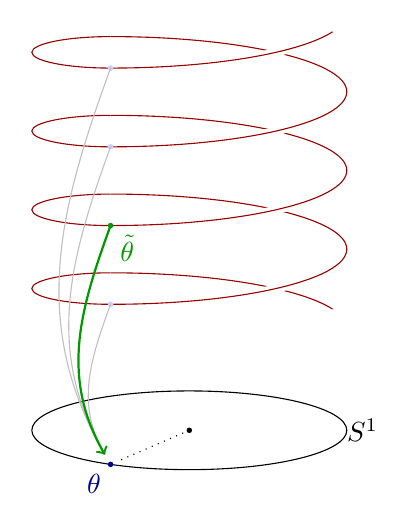
\begin{tikzpicture}[scale=1]
    \node[] (zero) at (0,0) {};
    \fill (zero) circle (1pt);
    \draw (0,-0.5) arc (270:-90:2 and 0.5);

    \node (theta) at ({cos(240) * 2},{sin(240) * 0.5}) {};
    % \node [below left of=theta,blue!40!white] {$\theta$};

    \draw[dotted] (0,0) -- (theta);
    \fill[blue!60!black] (theta) circle (1pt);


    \draw[red!60!black] (-1,2) arc (270:200:-3 and -0.7);
    \draw[line width=3pt,white] (-1,2) arc (270:90:1 and -0.2) arc (270:90:-3 and 0.7);
    \draw[red!60!black] (-1,2) arc (270:90:1 and -0.2) arc (270:90:-3 and 0.7);
    \fill[blue!20!white] (-1,1.6) circle (1pt);

    \draw[line width=3pt,white] (-1,3) arc (270:90:1 and -0.2) arc (270:90:-3 and 0.7);
    \draw[red!60!black] (-1,3) arc (270:90:1 and -0.2) arc (270:90:-3 and 0.7);
    \fill[green!60!black] (-1,2.6) circle (1pt);

    \draw[line width=3pt,white] (-1,4) arc (270:90:1 and -0.2) arc (270:90:-3 and 0.7);
    \draw[red!60!black] (-1,4) arc (270:90:1 and -0.2) arc (270:90:-3 and 0.7);
    \fill[blue!20!white] (-1,3.6) circle (1pt);

    \draw[line width=3pt,white] (-1,5) arc (270:90:1 and -0.2) arc (270:200:-3 and 0.7);
    \draw[red!60!black] (-1,5) arc (270:90:1 and -0.2) arc (270:200:-3 and 0.7);
    \fill[blue!20!white] (-1,4.6) circle (1pt);


    \draw[->,gray!50!white] (-1,1.6) to[out=250,in=120] (theta);
    \draw[->,gray!50!white] (-1,3.6) to[out=250,in=120] (theta);
    \draw[->,gray!50!white] (-1,4.6) to[out=250,in=120] (theta);
    \draw[->,green!60!black,thick] (-1,2.6) to[out=250,in=120] (theta);
    \node[below left,blue!60!black] at (theta) {$\theta$};
    \node[below right,green!60!black] at (-1,2.6) {$\tilde\theta$};

    \node[red!60!black] at (2.2,4.8) {$\R$};
    \node at (2.2,0) {$S^1$};
  \end{tikzpicture}
\end{center}

\textbf{$q$-sheet cover:}

\textbf{determination of a function:}
